\documentclass[12pt,preprint]{aastex}
\usepackage{listings}

\begin{document}

\title{Ay121 Lab Report Suggestions}

\tableofcontents

\section{Outline for a Scientific Paper}

\noindent
Below, we provide an outline of a typical scientific paper. This structure is only a suggested starting point. The content of a lab and your individual style make take you in
a different direct, which is fine. However you do it, though, a well-organized report is essential.

Within each of the sections described below, it is common to further divide content into subsections and
subsubsections, as warranted.  
Pay particular attention to sections 
 4, 5, and 6, which describe the data taking, 
analysis, and interpretation around which this course centers. 


\begin{enumerate}

\item \textbf{Title}:  Encapsulate the contents and meaning of the report.

\item \textbf{Abstract}: Briefly summary  the objectives, methods, and principal conclusions of the paper.  Tell a prospective reader whether it is worth spending time reading this article. Abstracts should contain essential information---{\it including the important numbers that you derive}.
  
\item \textbf{Introduction}: Set the context. Summarize the current state of
  knowledge, how that state can be improved, what this work does to
  advance the field.  The final sentences of the introduction should also map out the layout of the rest of the paper (e.g. ``In Section 2, we describe \dots; in Section 3, \dots" and so on).

\item \textbf{Methods}: Describe what you observed in enough detail that it can be reproduced. Note what equipment you used, how you recorded data, and any particulars or peculiarities.

\item \textbf{Data Analysis}: Describe the theoretical basis for your analysis,
  the analysis procedure, and the results of your analysis. Provide
  the essential numbers---the distillation of your original data (often
  millions of numbers) into a set of take-home results. This is
  what we mean by ``data reduction''!

\item \textbf{Interpretation}: Determine what the results mean in terms of astrophysics or
  your previous state of knowledge. How do your results relate to specific
  issues that were mentioned in the introduction? Compare the results you achieved with theoretical expectations and explore any deviations. Describe problems or difficulties that may affect your interpretation, as well as aspects that remain confusing or unclear.
 
\item \textbf{Conclusion}: Summarize the important results, pointing to particular sections as necessary. What aspects are lacking? How would
  you have done things better? Discuss prospects for future work.
  

\end{enumerate}

\section{Writing The Report}

\noindent
A blank is intimidating. Start with an outline---you can use the one above in \S1 to get you started. When you have sketched an outline, you have a map of where you are going and a way to estimate how much time and effort will be needed to finish your task.
\begin{itemize}
\item Set out your thoughts in an outline that organizes and directs the logical flow from introduction to conclusions. 
\item Some people write outlines and then fill in the details as they proceed. Others may or may not follow the outline, or even consult it as they write; however, thinking through the structure and logic of your report focuses your writing and leads to text that is easier to read. The first outline does not have to be complete---you can refine and expand it as you proceed. 
\item Once you have an outline, you do not have to work sequentially from start to finish. You can start the outline before you complete the experiment. Even if you do not know what your conclusions are you can still write a bullet that says ``Conclusions.”
\item Clear thinking precedes clear writing. The clearer the ideas are in your head, the clearer they will be on the page. However, it can often help to write something badly to clarify your thinking, then edit it so best say what you want to say.
\item Be explicit and transparent. A lab report is not a drama with plot twists. State (and re-state) your objectives, methods, and organization. 
\item State the principal results, both the intermediate ones and the final ones. Results are not just a table of numbers---describe the results in the text. Although a table may contain the actual answer, the reader will need help interpreting these results. 
\item Do not quote numbers without stating the uncertainty and the units.

\end{itemize}

\noindent
When you write your report, keep in mind who your reader is. As for any scientific writing, she is a critical (but not antagonistic) scientist. While you do not need to explain the science method or write down all the algebra that goes from one equation to the next, you need to convince her that at each step you have likely done the right thing. In the case of equation derivations, for instance, you may spell out one critical step (or approximation).


\section{Scientific and Interpretive Issues}

\noindent
These sections are {\it most important} because they related directly to
your scientific and experimental work and interpretation.
Overall, to make your work {\it science} it is important to
be self-critical. Check your reality! 

Various forms
of reality check include the following (a limited list):
\begin{enumerate}

	\item Generate fake data. Run your software on them ({\it note
the plural use of ``data''!}) and check for consistency. 

	\item When doing a least-squares fit, plot the {\it data},
overplot the {\it fitted curve}, and plot the {\it residuals}. The data
and fitted curve should look similar. The residuals should exhibit no
systematic trends and should look like noise clustered around zero. If
not, why not?

	\item Before deriving a result with fancy numerical techniques
you should first make a guess, using your physical intuition, about what the
answer is. If your fancy numerical technique gives something wildly
different, then  \begin{enumerate}

	\item Your physical intuition is no good, which means you don't
understand the basic fundamentals. 

	\item Your numerical technique or software is no good.
\end{enumerate}

\noindent Which is it? (Or is it both?) Talk to people, ask
questions, or whatever, but {\it resolve these discrepancies!}

\end{enumerate}
\end{itemize}

\noindent
When you plot  data, look at the plot and think
          about what you see.  For example, when observing the Sun with
          the interferometer on Campbell Hall's roof, the Campanile
          shadowed the dishes and the signal went away for some time.
          Ask yourself: what happened to the data during that time? In
          your lab report, such things are worth comments!


\section{Style}

\noindent
A lab report is a narrative recording your activities. In a lot of writing, style is an important consideration. Clarity trumps style in scientific writing; the clearer your report, the easier it will be for the reader to understand and follow your logic and writing. If you cannot explain what you have done clearly, it probably means that you do not understand it either—and you certainly will not convince anyone else that you know what you are describing. Some tips for clear writing include:
\begin{itemize}
\item Work from a plan or outline! You may find it helpful to flesh out each item in your outline into several concrete subtopics. Each major topic in your outline will likely deserve a section or subsection heading in your report. Use subsections to refine your direction and purpose.
\item Organize your thoughts into paragraphs. Use a topic sentence to focus each paragraph so that reader knows what is coming next.  Generally, people tend to write overly long paragraphs. Break them up!
\item Keep it simple. Write to express, not to impress! This means writing in short, simple sentences using common vocabulary and syntax. Use simple verbs and place them next to their subjects. Do not get tied down in complex clauses or language that may be ambiguous (e.g., double negatives can be ideal in some situations but tricky to read – do not make the reader re-read your sentences three times over!).
\item Brevity enhances clarity. Try to convey the maximum information in the minimum number of words. Avoid wordiness—eliminate unnecessary determiners and modifiers (aim at removing every instance of “very”, “somewhat”, “extremely”. “rather”, …); change phrases into single words; change unnecessary “that”, “who”, and “which” clauses into phrases; use active rather than passive verbs; replace circumlocutions with direct expressions. Watch out for weasel words and phrases, e.g., “it is known that… ,” “experience shows … .”
\item Read what your write and seek criticism! Talk about your ideas with others at different stages of writing your report. Get your roommate, lab partner, TA, professor, friend, sibling, or parent, to read your work. Remember, you should be your own severest critic. Finish your lab report a day early (!) and then reread at least eight hours later.
\item Conventional spelling and grammar counts. Scientific readers have very little patience with poor English and it will distract them from the scientific point you are trying to make. Use the sll checker, capitalize proper names, remember that 'data' is \emph{plural} in most contexts (use it as you would use the word 'datapoints').
\item Avoid colloquial and informal language. Don’t use contractions! Use acronyms sparingly, and define them on first use. If you have over 10 acronyms used frequently in your paper, consider making a glossary of terms to be placed before the introduction.
\item The format of this section notwithstanding, {\it use bullets sparingly}! Save them for making important points.
\end{itemize}

\section{Equations, Python, and Plots} \label{plotting}

\subsection{Equations}

\noindent
Equations, figures, and tables are key elements of your report. In the main body of the report, show all relevant equations that you used. Equations should be labeled with equation numbers so that you can refer to them in the text. If you quote an equation without derivation, cite the reference. 

Use equations as you present the explanation of what you did. When you include an equation, the text preceding and following it will explain in words what the equation means. Equations are delineated by punctuation because they are part of sentences. For example, put a period after an equation if it ends a sentence. The text preceding or following an equation should always define any new symbolic quantities that are used for the first time.

\subsection{Plotting and Python}

\noindent
Axis labels and annotations on plots need to be large
enough to be legible.  Also, use nice fonts. Don't
underestimate the value of good looks! Figure \ref{simple} illustrates
the difference between the following two plotting routines.

\lstinputlisting[language=Python]{plot_simple.py}

\lstinputlisting[language=Python]{plot_nicer.py}

\begin{figure}[htb]
\begin{center} 
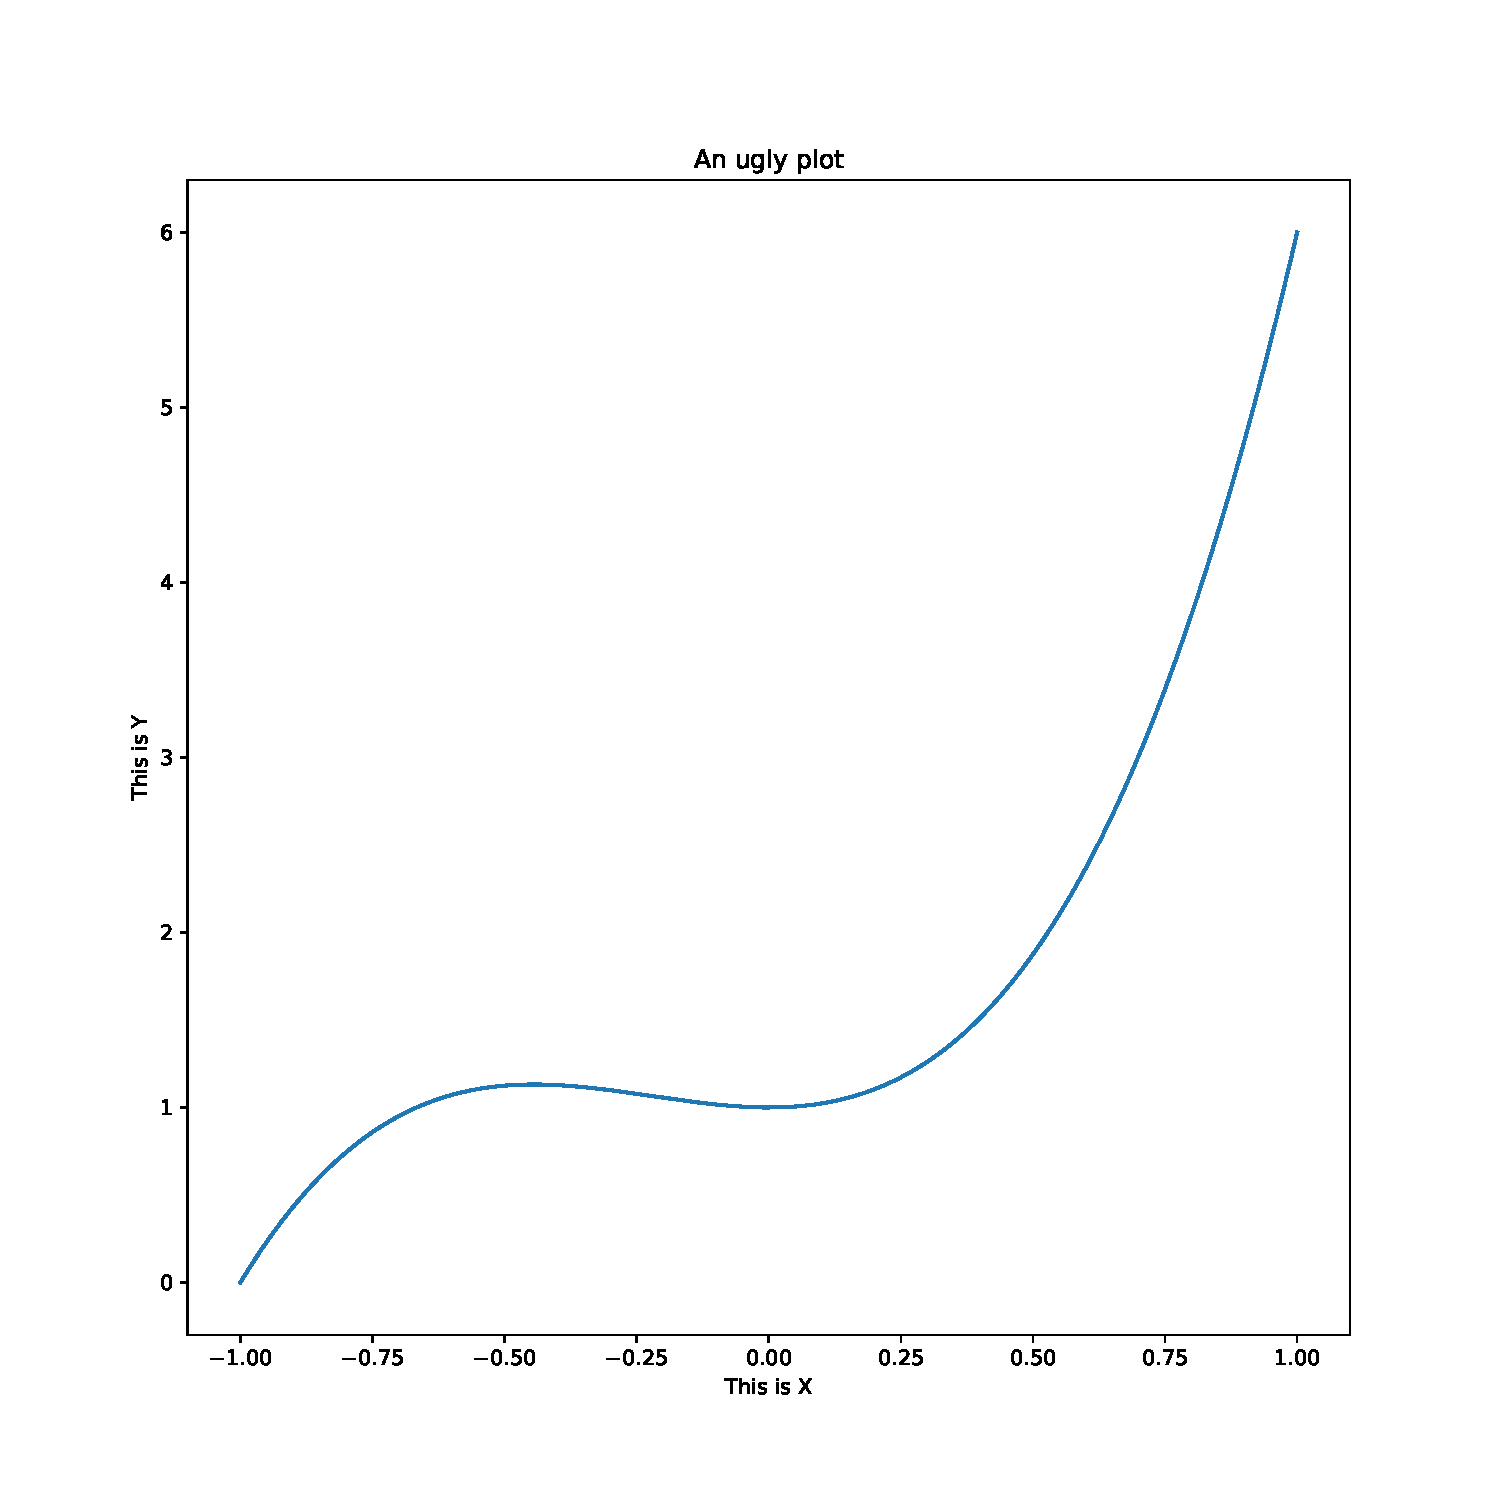
\includegraphics[width=3in]{simple.pdf}
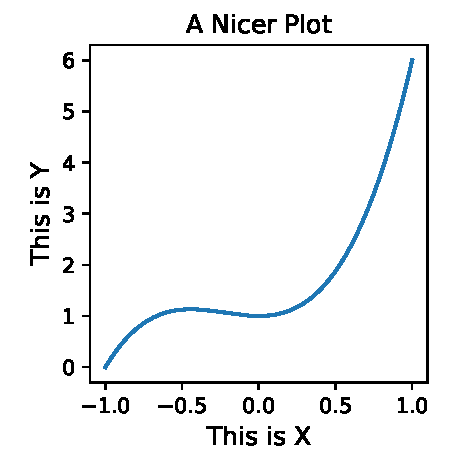
\includegraphics[width=3in]{nicer.pdf}
\end{center}
\caption{Left: Titles are too small, lines too thin, font doesn't look
good. Right: Nicer! (But it could be even nicer!) See \S
\ref{plotting}.  \label{simple}}
\end{figure}

When a plot is used in a paper, it should generally not have a title. Put anything you would have put in the title in the caption and make sure it is descriptive!

Make sure to reference your figure elsewhere in the paper than where you put it in. Figures will not necessarily be put in the correct place or ordering, so always use "Figure \textbackslash ref\{fig:A\}" to reference a figure in your text and "\textbackslash label\{fig:A\}" in the body of the figure so latex can fill in the correct number.

When plotting data, it's usually a good idea to plot the
  points themselves, which you'd do with the keyword \verb$marker='o'$, for
  example \footnote{Or any other symbol matplotlib supports}
    Sometimes you also want to connect the data points
  with lines, which you do with \verb$linestyle='solid'$.

When you do a least squares fit, you want to plot the
  data with a fitted curve; to do this, plot the data points
  (e.g.\ {\tt plot(x, data, 'ko')}) and then plot the fit over it
  in color (e.g.\ {\tt plot(x, fit, 'r-')}), but almost 20\% of human males are red/green
  colorblind, so out of consideration you should use a
  different line style (e.g.\ {\tt plot(x, fit, 'k--')}) or both
  ({\tt plot(x, fit, 'r--')}).


Python's matplotlib is able to use TeX markup.  This means you can put TeX into
titles and axis labels: (e.g. {\tt xlabel(r'\$\verb$\$nu\$ [MHz]')}).  Because '\verb$\$'
is an escape character in Python strings, you'll either need to use a double backslash (\verb$'\\nu'$)
or use raw strings (\verb$r'\nu'$).

Include detailed captions for all of your plots and figures. What do the points or curves represent? What does this graph reveal? What are some reasons this graph isn't perfect? A reader should be able to understand a graph just by reading the abstract, introduction, and its caption.

Finally, \textbf{avoid putting verbatim Python in your lab Report!} Explain your analysis in words so that the reader can reproduce it in their own way if they choose.

\section{TEX hints}

\noindent
Below are various TeX hints. This section is meant as a starting point; online tutorials can help you learn
how to format tables and other fancy things. LaTex is not always easy, but it is {\it powerful}.

\begin{enumerate}

	\item Mathematical convention says: usually, write
$(R^2-x^2)^{1/2}$ instead of $\sqrt{R^2-x^2}$.  In TEX, the scripts are
\verb&$(R^2-x^2)^{1/2}$& and \verb&$\sqrt{R^2-x^2}$&. 

	\item When you're doing complicated parenthetical expressions,
it's nice to use embedded sizing. TEX does this automatically for you:
instead of the not-very-elegant

$$x=\cos[2\pi(\frac{B_y}{\lambda}\cos(\delta))\sin(h)]$$

\noindent you can write

$$x=\cos\left[2\pi\left(\frac{B_y}{\lambda}\cos(\delta)\right)\sin(h)\right]$$

\noindent The scripts for these are

\begin{verbatim} 
$$x=\cos[2\pi(\frac{B_y}{\lambda}\cos(\delta))\sin(h)]$$

and

$$x=\cos\left[2\pi\left(\frac{B_y}{\lambda}\cos(\delta)\right)\sin(h)\right]$$
\end{verbatim}

\noindent Note the (double) use of \verb$\left[$ and \verb$\right$] . 
Also, note the Roman letters for the trig function, i.e.\ convention
prefers $\cos(ha)$ instead of $cos(ha)$; we accomplish this in TEX by
writing \verb$\cos(ha)$ (note backwards slash in \verb$\cos$) instead of
\verb$cos(ha)$. 

\item You can print a Table of Contents by writing
\verb$\tableofcontents$ in your TEX document (usually at the beginning,
but you can do it anywhere). This is very helpful when
organizing your lab report into sections and subsections.

\item You can get the proper looking quotes, either `single' or
``double'', by writing \verb$`single'$ or \verb$``double''$ . 

\item You can get a proper ``times'' sign, as in $2 \times 3$, using
\verb=$2 \times 3$=. 

\item You can get equations numbered 1a, 2b, and 3c instead of 4, 5,
and 6 by using the \verb$mathletters$ environment like this:
\begin{mathletters}
\begin{equation}
x = \sin (y)
\end{equation}
\noindent and then you can insert as much text as you want and\dots
\begin{equation}
z = \tan (y)
\end{equation}
\begin{equation}
u =  y^{1/2}
\end{equation}
\end{mathletters}
by typing the following:
\begin{verbatim}
\begin{mathletters}
\begin{equation}
x = \sin (y)
\end{equation}

\noindent and then you can insert as much text as you want and\dots

\begin{equation}
z = \tan (y)
\end{equation}
\begin{equation}
u =  y^{1/2}
\end{equation}
\end{mathletters}
\end{verbatim}

\item And finally, you can insert things verbatim into TEX, without the
TEX translations, by using \verb=\verb$verbatim into TEX$= (all must be
on one line) or, for multiple lines, get into the \verb$verbatim$
environment by typing

\begin{verbatim}
\begin{verbatim}
Now we are in the verbatim environment
Here is a multiple line situation
\end{verbatim}
\verb$\end{verbatim}$
\end{enumerate}

\section{Grades}

\noindent
 Convince me that you understand
 what you are doing.  Look at the list of goals in the lab handout and try to address each goal. Then look at the above sections in this
 handout and incorporate them in your report.

When covering a given topic, include supporting data with figures,
 tables, and discussion to the extent that they are illustrative and
 educational for the reader. Don't include material simply because `it's
 there' or to make your report longer. What matters is clarity. Being concise is a virtue. Instead of including every
 plot you made, a well-considered and
 well-selected subset of plots---annotated, labelled, presented neatly, and
discussed in the text---shows that you understand what is important.

If your results seem discrepant with expectation, how do you resolve
this? You might think that  you have to `get the right answer', But in
research, particularly experimental research, the `right answer' may
differ depending on the experimental conditions, such as signal levels
or interfering signals. Should you hide or minimize your puzzlements or
mistakes so that I'll think you're really smart? Or should you emphasize
your problems or difficulties by showing them explicitly, sometimes
even to the extent of having a separate section that discusses them?
Which way will you learn more? Which way will I appreciate?

Finally, if you can make your report interesting to me as a reader, then that in
 itself can be a marker of your  understanding. 
 
 \subsection{Rubric}
 
 \noindent
 Broadly, reports will be graded according to the following rubric:
 \begin{enumerate}
     \item Format (5 points). Report does not exceed 10 pages (including tables and figures) in 12 pt font. Spelling and grammar are correct. Title, date, name, group, and division of labor are all displayed.
     \item Abstract (5 points). It should succinctly state the objectives, methods, and principal conclusions of the experiment.
     \item Introduction (10 points). It should concisely motivate the problem and introduce the methods used to pursue its solution.
     \item Observations and Data (5 points). Report describes the equipment used, how data were acquired, and anomalies or systematic errors that may be present in the data.
     \item Data Reduction and Manipulation (5 points). Report should describe data reduction methods/algorithms and statistical methods used to analyze the data. The reader is adequately led through intermediate to final results with each step clearly explained.
     \item Calculations and Modeling (10 points). Report should demonstrate complete understanding of the physical principles underlying the experiment. Intermediate calculations with plots or tables appear in a logical sequence throughout and are sufficient to convince the reader that the final results are correct. All equations used appear in the text with equation numbers and references. Equations are described and explained as part of sentences within the context of the experiment, and all new symbolic quantities are defined. Figures and tables have clear captions, numbers, and labels, are referred to in the body of the report, are placed in the text close to where they are referenced, and are used to support key arguments in the text.
     \item Discussion (10 points). Report synthesizes, analyzes, and interprets the results in the context of the experimental purpose. Results are compared with theoretical expectations. Discrepancies between theory and results are explained appropriately in terms of errors in measurement and technique. Describes remaining ambiguities, uncertainties, and avenues for future investigation. Includes an insightful summary of conclusions.
     \item Structure and Style (10 points). The lab report has narrative drive. The overall goal and methods are clear from the beginning and serve as a key driver throughout the text. The report follows a logical structure on all scales, from sentences, to paragraphs, to subsections, to sections, and conveys the  information concisely. The activities described demonstrate initiative and creativity on the part of the individual. 
 \end{enumerate}

\end{document}
